% !TEX spellcheck = en_US

\documentclass[aspectratio=169,10pt,compress]{beamer}

% ~~~~~~~~~~~~~~~~~~~~~~~~~~~~~~~~~~~~~~~~~~~~~~~~~~~~~~~~~~~~~~ V beamer
	\useoutertheme{split}
	\useinnertheme{rounded}
	\usecolortheme{whale}
	\usecolortheme{orchid}
	\setbeamertemplate{blocks}[rounded]
	\setbeamertemplate{navigation symbols}{}
	\setbeamertemplate{page number in head/foot}[totalframenumber]
	% "i / N" on every frame comes from hblibPresentation.sty (\insertshorttitle)
% ~~~~~~~~~~~~~~~~~~~~~~~~~~~~~~~~~~~~~~~~~~~~~~~~~~~~~~~~~~~~~~ V beamer



% ~~~~~~~~~~~~~~~~~~~~~~~~~~~~~~~~~~~~~~~~~~~~~~~~~~~~~~~~~~~~~~ V hblib
	\usepackage{../../hblib/hblibPresentation} % lib presentation 
	\usepackage{../../hblib/hblibCodeoutput} % lib code listing
% ~~~~~~~~~~~~~~~~~~~~~~~~~~~~~~~~~~~~~~~~~~~~~~~~~~~~~~~~~~~~~~ A hblib


\usepackage[T1]{fontenc}
\usepackage{lmodern}
\usepackage{listings}
\usepackage{xcolor}
\usepackage{booktabs}
\usepackage{array}
\usepackage{tikz}
\usetikzlibrary{positioning,arrows.meta,calc}

\newcolumntype{L}[1]{>{\raggedright\arraybackslash}p{#1}}

\definecolor{codebg}{RGB}{245,245,245}
\definecolor{codecomment}{RGB}{110,110,110}
\definecolor{gitred}{RGB}{240,80,50}
\definecolor{gitblue}{RGB}{40,90,160}
\definecolor{gitgreen}{RGB}{40,130,70}

\lstset{
  language=bash,
  basicstyle=\ttfamily\footnotesize,
  backgroundcolor=\color{codebg},
  commentstyle=\color{codecomment}\itshape,
  keywordstyle=\color{gitred}\bfseries,
  morekeywords={git},
  frame=single,
  rulecolor=\color{gray!40},
  columns=fullflexible,
  keepspaces=true,
  showstringspaces=false,
  breaklines=true,
  xleftmargin=4pt,
  xrightmargin=4pt,
  aboveskip=4pt,
  belowskip=4pt
}

\newcommand{\cmd}[1]{\texttt{\color{gitred}#1}}

\tikzset{
  commit/.style={circle, draw=gitblue, fill=gitblue!15, thick, minimum size=7mm,
                 inner sep=0pt, font=\scriptsize\ttfamily},
  newcommit/.style={commit, draw=gitred, fill=gitred!15},
  edge/.style={-{Stealth[length=2mm]}, thick, gray!70},
  lbl/.style={font=\scriptsize\bfseries, text=gitred},
  ref/.style={draw=gitred, thick, fill=gitred!12, rounded corners=2pt,
              font=\scriptsize\ttfamily, inner sep=2pt},
  headref/.style={ref, draw=gitblue, fill=gitblue!12},
  ptr/.style={-{Stealth[length=1.6mm]}, thick, gitred}
}

\title{Git for Sophomores}
\subtitle{Working Together in a Shared Repository}
\author[Bingol]{Haluk O. Bingol}

\institute[FCIS]{
    Faculty of Computer and Information Sciences\\
    Yeditepe University
}
\date{
	{\tiny \hbTimeStamp}
}

\begin{document}

% ~~~~~~~~~~~~~~~~~~~~~~~~~~~~~~~~~~~~~~ V
\begin{frame}[t,fragile]
  \titlepage
\end{frame}
% ~~~~~~~~~~~~~~~~~~~~~~~~~~~~~~~~~~~~~~ A

% ~~~~~~~~~~~~~~~~~~~~~~~~~~~~~~~~~~~~~~ V
\begin{frame}[t,fragile] \frametitle{Outline}
  \begin{columns}[T]
    \begin{column}{0.5\textwidth}
      \tableofcontents[sections={1-5}]
    \end{column}
    \begin{column}{0.5\textwidth}
      \tableofcontents[sections={6-10}]
    \end{column}
  \end{columns}
\end{frame}
% ~~~~~~~~~~~~~~~~~~~~~~~~~~~~~~~~~~~~~~ A

% ~~~~~~~~~~~~~~~~~~~~~~~~~~~~~~~~~~~~~~ V
\begin{frame}[t,fragile] \frametitle{Where we are}
  \textbf{You already know} (freshman level):
  \begin{itemize}
    \item \cmd{init}, \cmd{add}, \cmd{commit}, \cmd{status}, \cmd{log}, \cmd{diff}
    \item branches: \cmd{switch -c}, \cmd{merge}, resolving a simple conflict
    \item \cmd{clone}, \cmd{pull}, \cmd{push}, \texttt{.gitignore}, basic undo
  \end{itemize}

  \vspace{0.5em}
  \textbf{This lecture:} from \emph{one person, one laptop} to \emph{a team, one repository}
  \begin{itemize}
    \item understand what Git is really doing when you branch, pull and push
    \item work with 3--4 teammates without breaking each other's code
    \item use GitHub to plan, review and track the work
  \end{itemize}

  \vspace{0.5em}
  \begin{block}{Goal}
    By the end of the term, your team's \texttt{main} always builds and every
    change arrived through a reviewed pull request.
  \end{block}
\end{frame}
% ~~~~~~~~~~~~~~~~~~~~~~~~~~~~~~~~~~~~~~ A

% ~~~~~~~~~~~~~~~~~~~~~~~~~~~~~~~~~~~~~~ V
\section[Model]{A Better Mental Model}
% ~~~~~~~~~~~~~~~~~~~~~~~~~~~~~~~~~~~~~~ A

% ~~~~~~~~~~~~~~~~~~~~~~~~~~~~~~~~~~~~~~ V
\begin{frame}[t,fragile] \frametitle{Commits form a graph; branches are labels}
  \begin{center}
  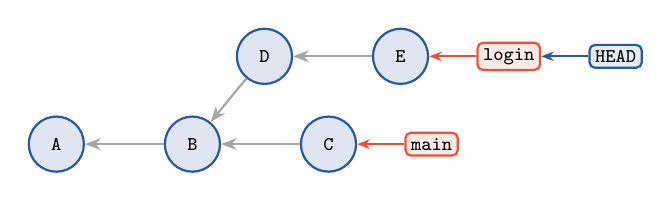
\begin{tikzpicture}[node distance=10mm]
    \node[commit] (a) {A};
    \node[commit, right=of a] (b) {B};
    \node[commit, right=of b] (c) {C};
    \node[commit, above right=6mm and 4mm of b] (d) {D};
    \node[commit, right=of d] (e) {E};
    \draw[edge] (b) -- (a); \draw[edge] (c) -- (b);
    \draw[edge] (d) -- (b); \draw[edge] (e) -- (d);
    \node[ref, right=6mm of c] (main) {main};
    \node[ref, right=6mm of e] (feat) {login};
    \node[headref, right=6mm of feat] (head) {HEAD};
    \draw[ptr] (main) -- (c); \draw[ptr] (feat) -- (e);
    \draw[ptr, gitblue] (head) -- (feat);
  \end{tikzpicture}
  \end{center}

  \begin{itemize}
    \item A \textbf{commit} is a full snapshot of the project, plus a link to its parent(s)
    \item A \textbf{branch} is just a movable label pointing at one commit
    \item \textbf{HEAD} says ``where you are'': normally it points at a branch
    \item When you commit, the branch HEAD points to moves forward to the new commit
  \end{itemize}

\begin{lstlisting}
git log --oneline --graph --all    # draw this picture for your own repo
\end{lstlisting}
\end{frame}
% ~~~~~~~~~~~~~~~~~~~~~~~~~~~~~~~~~~~~~~ A

% ~~~~~~~~~~~~~~~~~~~~~~~~~~~~~~~~~~~~~~ V
\begin{frame}[t,fragile] \frametitle{Detached HEAD: what it is and how to get out}
  If HEAD points directly at a commit instead of a branch, you are in \textbf{detached HEAD}:
\begin{lstlisting}
git switch --detach a1b2c3d       # look at an old version
# HEAD is now at a1b2c3d Add data model
\end{lstlisting}

  \begin{columns}[T]
    \begin{column}{0.48\textwidth}
      \textbf{Just looking?} Go back:
\begin{lstlisting}
git switch main
\end{lstlisting}
    \end{column}
    \begin{column}{0.48\textwidth}
      \textbf{Made commits you want to keep?}
\begin{lstlisting}
git switch -c rescue-work
\end{lstlisting}
    \end{column}
  \end{columns}

  \vspace{0.5em}
  \begin{alertblock}{Why it matters}
    Commits made in detached HEAD belong to no branch. If you switch away without
    creating one, they become hard to find.
  \end{alertblock}
\end{frame}
% ~~~~~~~~~~~~~~~~~~~~~~~~~~~~~~~~~~~~~~ A

% ~~~~~~~~~~~~~~~~~~~~~~~~~~~~~~~~~~~~~~ V
\begin{frame}[t,fragile] \frametitle{Fast-forward vs.\ merge commit}
  \begin{columns}[T]
    \begin{column}{0.48\textwidth}
      \centering\textbf{Fast-forward}\\[2pt]
      \small \texttt{main} has no new commits\\[4pt]
      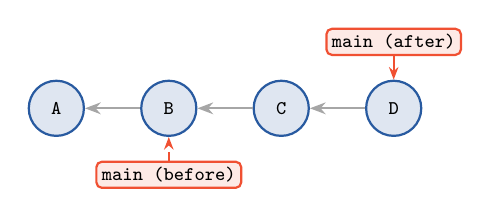
\begin{tikzpicture}[node distance=7mm]
        \node[commit] (a) {A};
        \node[commit, right=of a] (b) {B};
        \node[commit, right=of b] (c) {C};
        \node[commit, right=of c] (d) {D};
        \draw[edge] (b) -- (a); \draw[edge] (c) -- (b); \draw[edge] (d) -- (c);
        \node[ref, below=3mm of b] (m0) {main (before)};
        \node[ref, above=3mm of d] (m1) {main (after)};
        \draw[ptr, dashed] (m0) -- (b); \draw[ptr] (m1) -- (d);
      \end{tikzpicture}\\[4pt]
      \small The label just slides forward.\\ No new commit is created.
    \end{column}
    \begin{column}{0.48\textwidth}
      \centering\textbf{Merge commit}\\[2pt]
      \small both branches have new commits\\[4pt]
      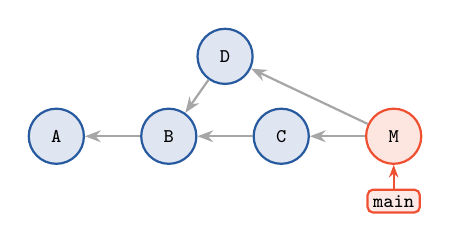
\begin{tikzpicture}[node distance=7mm]
        \node[commit] (a) {A};
        \node[commit, right=of a] (b) {B};
        \node[commit, right=of b] (c) {C};
        \node[commit, above right=5mm and 2mm of b] (d) {D};
        \node[newcommit, right=of c] (m) {M};
        \draw[edge] (b) -- (a); \draw[edge] (c) -- (b); \draw[edge] (d) -- (b);
        \draw[edge] (m) -- (c); \draw[edge] (m) -- (d);
        \node[ref, below=3mm of m] (mm) {main};
        \draw[ptr] (mm) -- (m);
      \end{tikzpicture}\\[4pt]
      \small \texttt{M} has \textbf{two parents}.\\ Conflicts can happen here.
    \end{column}
  \end{columns}

  \vspace{0.5em}
\begin{lstlisting}
git merge --ff-only feature       # merge only if it can fast-forward
git merge --no-ff feature         # always create a merge commit
\end{lstlisting}
\end{frame}
% ~~~~~~~~~~~~~~~~~~~~~~~~~~~~~~~~~~~~~~ A

% ~~~~~~~~~~~~~~~~~~~~~~~~~~~~~~~~~~~~~~ V
\section[Remotes]{Remotes, Properly}
% ~~~~~~~~~~~~~~~~~~~~~~~~~~~~~~~~~~~~~~ A

% ~~~~~~~~~~~~~~~~~~~~~~~~~~~~~~~~~~~~~~ V
\begin{frame}[t,fragile] \frametitle{Three copies of \texttt{main}}
  \begin{center}
  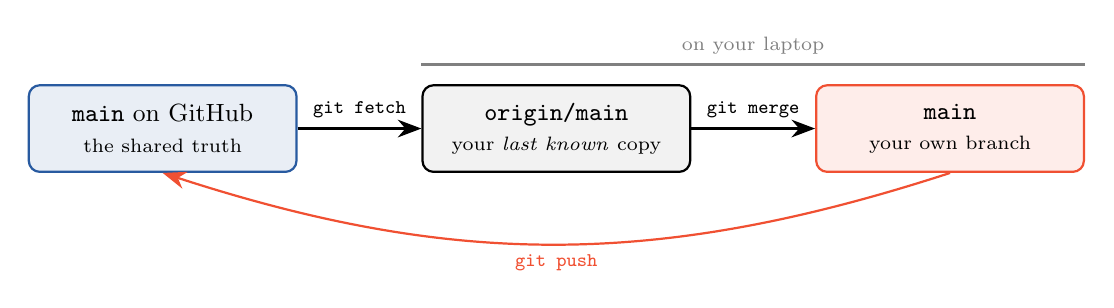
\begin{tikzpicture}[
      box/.style={draw, rounded corners, thick, minimum width=3.4cm, minimum height=1.1cm,
                  align=center, font=\small},
      arr/.style={-{Stealth[length=3mm]}, thick}]
    \node[box, fill=gitblue!10, draw=gitblue] (gh) at (0,0)
         {\texttt{main} on GitHub\\ \scriptsize the shared truth};
    \node[box, fill=gray!10] (om) at (5,0)
         {\texttt{origin/main}\\ \scriptsize your \emph{last known} copy};
    \node[box, fill=gitred!10, draw=gitred] (lm) at (10,0)
         {\texttt{main}\\ \scriptsize your own branch};
    \draw[arr] (gh) -- node[above, font=\scriptsize\ttfamily]{git fetch} (om);
    \draw[arr] (om) -- node[above, font=\scriptsize\ttfamily]{git merge} (lm);
    \draw[arr, gitred] (lm.south) to[bend left=18] node[below, font=\scriptsize\ttfamily]{git push} (gh.south);
    \draw[thick, gray] ($(om.north west)+(0,0.25)$) -- ($(lm.north east)+(0,0.25)$)
          node[midway, above, font=\scriptsize]{on your laptop};
  \end{tikzpicture}
  \end{center}

  \vspace{-0.5em}
  \begin{itemize}
    \item \texttt{origin/main} is a \textbf{remote-tracking branch}: read-only, updated only by \cmd{fetch}
    \item \cmd{git pull} = \cmd{git fetch} + \cmd{git merge origin/main}
    \item \cmd{git fetch} is always safe: it never touches your files
  \end{itemize}
\end{frame}
% ~~~~~~~~~~~~~~~~~~~~~~~~~~~~~~~~~~~~~~ A

% ~~~~~~~~~~~~~~~~~~~~~~~~~~~~~~~~~~~~~~ V
\begin{frame}[t,fragile] \frametitle{Tracking branches: ahead and behind}
\begin{lstlisting}
git push -u origin login          # -u: "login" now tracks "origin/login"
git branch -vv                    # show what each branch tracks
#  * login  7c1d9e2 [origin/login: ahead 2] Add password check
#    main   4a5b6c7 [origin/main: behind 3] Update README

git fetch                         # refresh origin/* first, then:
git status
#  Your branch and 'origin/main' have diverged,
#  and have 2 and 3 different commits each, respectively.
\end{lstlisting}

  \small
  \begin{tabular}{@{}L{0.25\textwidth}L{0.65\textwidth}@{}}
    \toprule
    \textbf{Status} & \textbf{What to do} \\
    \midrule
    ahead      & you have unpushed commits: \cmd{git push} \\
    behind     & teammates pushed: \cmd{git pull} \\
    diverged   & both: \cmd{git pull} (merge), resolve conflicts, then \cmd{git push} \\
    \bottomrule
  \end{tabular}
\end{frame}
% ~~~~~~~~~~~~~~~~~~~~~~~~~~~~~~~~~~~~~~ A

% ~~~~~~~~~~~~~~~~~~~~~~~~~~~~~~~~~~~~~~ V
\begin{frame}[t,fragile] \frametitle{``Push rejected'': don't panic, don't force}
\begin{lstlisting}[language={}]
$ git push
 ! [rejected]        main -> main (fetch first)
error: failed to push some refs to 'github.com:team/app.git'
hint: Updates were rejected because the remote contains work that you
hint: do not have locally.
\end{lstlisting}

  \textbf{What happened:} a teammate pushed first. GitHub refuses a push that would
  throw away their commits.

\begin{lstlisting}
git pull                          # bring in their work (resolve conflicts if any)
# run the tests!
git push                          # now it succeeds
\end{lstlisting}

  \begin{alertblock}{Never ``fix'' this with \texttt{git push --force}}
    Forcing overwrites GitHub with your copy and \textbf{deletes your teammates' commits}.
  \end{alertblock}
\end{frame}
% ~~~~~~~~~~~~~~~~~~~~~~~~~~~~~~~~~~~~~~ A

% ~~~~~~~~~~~~~~~~~~~~~~~~~~~~~~~~~~~~~~ V
\section[Teamwork]{Team Workflow in a Shared Repo}
% ~~~~~~~~~~~~~~~~~~~~~~~~~~~~~~~~~~~~~~ A

% ~~~~~~~~~~~~~~~~~~~~~~~~~~~~~~~~~~~~~~ V
\begin{frame}[t,fragile] \frametitle{Setting up the team repository}
  \begin{enumerate}
    \item One person creates the repo on GitHub, with a \texttt{README}, \texttt{.gitignore} and \texttt{LICENSE}
    \item \textbf{Settings $\rightarrow$ Collaborators}: invite every teammate (and the instructor)
    \item \textbf{Settings $\rightarrow$ Branches}: add a rule for \texttt{main}
      \begin{itemize}\small
        \item require a pull request before merging
        \item require at least 1 approval
      \end{itemize}
    \item Everyone clones the \emph{same} repo; no forks needed
  \end{enumerate}

  \vspace{0.5em}
  \begin{block}{The one rule}
    Nobody commits directly to \texttt{main}. Every change goes through a branch and a pull request.
  \end{block}
\end{frame}
% ~~~~~~~~~~~~~~~~~~~~~~~~~~~~~~~~~~~~~~ A

% ~~~~~~~~~~~~~~~~~~~~~~~~~~~~~~~~~~~~~~ V
\begin{frame}[t,fragile] \frametitle{The feature-branch loop}
\begin{lstlisting}
git switch main
git pull                              # 1. start from the latest main
git switch -c 12-search-by-name       # 2. one branch per issue
# ...edit, add, commit (small commits!)...
git push -u origin 12-search-by-name  # 3. publish the branch
# 4. open a pull request on GitHub; teammates review
# 5. while waiting, keep your branch up to date:
git fetch
git merge origin/main                 # resolve conflicts on YOUR branch
git push
# 6. after the PR is merged, clean up:
git switch main && git pull
git branch -d 12-search-by-name
\end{lstlisting}
  \small Tip: start branch names with the issue number, e.g.\ \texttt{12-search-by-name}.
\end{frame}
% ~~~~~~~~~~~~~~~~~~~~~~~~~~~~~~~~~~~~~~ A

% ~~~~~~~~~~~~~~~~~~~~~~~~~~~~~~~~~~~~~~ V
\begin{frame}[t,fragile] \frametitle{Pull requests and code review}
  \begin{columns}[T]
    \begin{column}{0.48\textwidth}
      \textbf{Opening a PR}
      \begin{itemize}\small
        \item Title says what changed
        \item Description says \emph{why} and how to test it
        \item Add \texttt{Closes \#12} to link the issue
        \item Request a reviewer
        \item Keep it small: under $\sim$300 lines
      \end{itemize}
      \vspace{0.3em}
      \textbf{Updating a PR}
      \begin{itemize}\small
        \item Push more commits to the same branch; the PR updates itself
      \end{itemize}
    \end{column}
    \begin{column}{0.48\textwidth}
      \textbf{Reviewing a PR}
      \begin{itemize}\small
        \item Read the diff in \emph{Files changed}
        \item Pull the branch and run it if needed
        \item Comment on specific lines
        \item \emph{Approve} or \emph{Request changes}
      \end{itemize}
      \vspace{0.3em}
      \textbf{Good review manners}
      \begin{itemize}\small
        \item Comment on the code, not the person
        \item Ask questions: ``What happens if the list is empty?''
        \item Say what's good, too
      \end{itemize}
    \end{column}
  \end{columns}
\end{frame}
% ~~~~~~~~~~~~~~~~~~~~~~~~~~~~~~~~~~~~~~ A

% ~~~~~~~~~~~~~~~~~~~~~~~~~~~~~~~~~~~~~~ V
\section[Conflicts]{Conflicts with Confidence}
% ~~~~~~~~~~~~~~~~~~~~~~~~~~~~~~~~~~~~~~ A

% ~~~~~~~~~~~~~~~~~~~~~~~~~~~~~~~~~~~~~~ V
\begin{frame}[t,fragile] \frametitle{Resolving a real conflict}
\begin{lstlisting}
git merge origin/main
# CONFLICT (content): Merge conflict in src/search.py
# CONFLICT (content): Merge conflict in README.md
git status                        # "both modified:" lists every conflicted file
\end{lstlisting}

  \begin{columns}[T]
    \begin{column}{0.55\textwidth}
      \textbf{For each file}
      \begin{enumerate}\small
        \item Open it; find every \texttt{<{}<{}<{}<{}<{}<{}<} block
        \item Keep ours, theirs, or write a combination
        \item Remove all conflict markers
        \item \cmd{git add <file>}
      \end{enumerate}
      \textbf{Then}
      \begin{enumerate}\small\setcounter{enumi}{4}
        \item \textbf{Build and run the tests}
        \item \cmd{git commit} to finish the merge
      \end{enumerate}
    \end{column}
    \begin{column}{0.42\textwidth}
      \begin{block}{Changed your mind?}
        \cmd{git merge --abort} puts everything back exactly as it was before the merge.
      \end{block}
      \begin{block}{In VS Code}
        \small Use \emph{Accept Current / Incoming / Both}, or
        \emph{Resolve in Merge Editor} for a 3-way view.
      \end{block}
    \end{column}
  \end{columns}
\end{frame}
% ~~~~~~~~~~~~~~~~~~~~~~~~~~~~~~~~~~~~~~ A

% ~~~~~~~~~~~~~~~~~~~~~~~~~~~~~~~~~~~~~~ V
\begin{frame}[t,fragile] \frametitle{Preventing conflicts}
  Conflicts are not errors. They happen when two people edit the same lines.
  You can make them rare and small:

  \vspace{0.5em}
  \begin{itemize}
    \item \textbf{Pull often.} Start every work session with \cmd{git pull}
    \item \textbf{Keep branches short-lived.} Merge within days, not weeks
    \item \textbf{Keep PRs small.} One issue per branch
    \item \textbf{Divide the work by file or module} when planning tasks
    \item \textbf{Talk.} ``I'm refactoring \texttt{search.py} today'' saves an hour of merging
    \item \textbf{Don't reformat whole files} in a feature branch; it changes every line
  \end{itemize}

  \vspace{0.5em}
  \begin{alertblock}{Silent conflicts}
    A merge can succeed and still break the program (e.g.\ one person renames a function
    another person just started calling). Always build and test after merging.
  \end{alertblock}
\end{frame}
% ~~~~~~~~~~~~~~~~~~~~~~~~~~~~~~~~~~~~~~ A

% ~~~~~~~~~~~~~~~~~~~~~~~~~~~~~~~~~~~~~~ V
\section[GitHub]{GitHub as a Project Tool}
% ~~~~~~~~~~~~~~~~~~~~~~~~~~~~~~~~~~~~~~ A

% ~~~~~~~~~~~~~~~~~~~~~~~~~~~~~~~~~~~~~~ V
\begin{frame}[t,fragile] \frametitle{Issues, labels and project boards}
  \begin{columns}[T]
    \begin{column}{0.5\textwidth}
      \textbf{Issues} are the team's to-do list
      \begin{itemize}\small
        \item one issue = one task or bug
        \item assign it to one person
        \item labels: \texttt{bug}, \texttt{feature}, \texttt{docs}
        \item milestones: ``Sprint 1'', ``Demo day''
      \end{itemize}
      \vspace{0.3em}
      \textbf{Project board}
      \begin{itemize}\small
        \item columns: \emph{Todo} $\rightarrow$ \emph{In progress} $\rightarrow$ \emph{Done}
        \item the whole team sees who is doing what
      \end{itemize}
    \end{column}
    \begin{column}{0.47\textwidth}
      \textbf{Linking code to issues}
\begin{lstlisting}[language={}]
Add search by student name

Closes #12
\end{lstlisting}
      \small
      When this commit or PR is merged into \texttt{main}, issue \#12 closes automatically.
      Also works with \texttt{Fixes} and \texttt{Resolves}.

      \vspace{0.3em}
      Mentioning \texttt{\#12} anywhere links back to the issue.
    \end{column}
  \end{columns}
\end{frame}
% ~~~~~~~~~~~~~~~~~~~~~~~~~~~~~~~~~~~~~~ A

% ~~~~~~~~~~~~~~~~~~~~~~~~~~~~~~~~~~~~~~ V
\begin{frame}[t,fragile] \frametitle{README and LICENSE}
  \begin{columns}[T]
    \begin{column}{0.52\textwidth}
\begin{lstlisting}[language={}]
# Grade Tracker

A command-line tool to track course grades.

## Setup
    pip install -r requirements.txt

## Usage
    python main.py add "CSE 211" 87

## Team
- Ayse Yilmaz: storage
- Mehmet Kaya: reports
\end{lstlisting}
    \end{column}
    \begin{column}{0.45\textwidth}
      \textbf{A README answers}
      \begin{itemize}\small
        \item What is this?
        \item How do I install and run it?
        \item Who made it, and how do I contribute?
      \end{itemize}
      \vspace{0.3em}
      \textbf{LICENSE}
      \begin{itemize}\small
        \item No license = nobody else may legally reuse your code
        \item \textbf{MIT}: short and permissive
        \item \textbf{GPL}: derivatives must stay open source
        \item Check your university's policy for course work
      \end{itemize}
    \end{column}
  \end{columns}
\end{frame}
% ~~~~~~~~~~~~~~~~~~~~~~~~~~~~~~~~~~~~~~ A

% ~~~~~~~~~~~~~~~~~~~~~~~~~~~~~~~~~~~~~~ V
\section[Setup]{Setup That Saves Pain Later}
% ~~~~~~~~~~~~~~~~~~~~~~~~~~~~~~~~~~~~~~ A

% ~~~~~~~~~~~~~~~~~~~~~~~~~~~~~~~~~~~~~~ V
\subsection[SSH keys]{SSH keys}
% ~~~~~~~~~~~~~~~~~~~~~~~~~~~~~~~~~~~~~~ A

% ~~~~~~~~~~~~~~~~~~~~~~~~~~~~~~~~~~~~~~ V
\begin{frame}[t,fragile] \frametitle{SSH keys: push without passwords}
\begin{lstlisting}
ssh-keygen -t ed25519 -C "you@university.edu"   # press Enter for defaults
cat ~/.ssh/id_ed25519.pub         # copy this PUBLIC key
# GitHub: Settings -> SSH and GPG keys -> New SSH key -> paste
ssh -T git@github.com             # "Hi you! You've successfully authenticated"

git clone git@github.com:team/app.git              # clone with SSH
git remote set-url origin git@github.com:team/app.git   # or switch an existing repo
\end{lstlisting}

  \begin{columns}[T]
    \begin{column}{0.48\textwidth}
      \begin{alertblock}{Private key stays private}
        Never share or commit \texttt{id\_ed25519} (no \texttt{.pub}).
      \end{alertblock}
    \end{column}
    \begin{column}{0.48\textwidth}
      \begin{block}{Two machines?}
        Make one key per machine (lab PC, laptop) and add each to GitHub.
      \end{block}
    \end{column}
  \end{columns}
\end{frame}
% ~~~~~~~~~~~~~~~~~~~~~~~~~~~~~~~~~~~~~~ A

% ~~~~~~~~~~~~~~~~~~~~~~~~~~~~~~~~~~~~~~ V
\subsection{Editor}
% ~~~~~~~~~~~~~~~~~~~~~~~~~~~~~~~~~~~~~~ A

% ~~~~~~~~~~~~~~~~~~~~~~~~~~~~~~~~~~~~~~ V
\begin{frame}[t,fragile] \frametitle{Editor, line endings and aliases}
\begin{lstlisting}
git config --global core.editor "code --wait"   # or "nano"; avoids the Vim trap
git config --global push.autoSetupRemote true  # first push needs no -u
git config --global alias.st status
git config --global alias.lg "log --oneline --graph --all"
git help merge                                  # full manual for any command
\end{lstlisting}

  \textbf{Line endings:} Windows uses CRLF, macOS/Linux use LF. In a mixed team, every
  line of a file can appear ``changed''. Fix it once, for the whole team:
  \begin{columns}[T]
    \begin{column}{0.4\textwidth}
\begin{lstlisting}[language={}]
# .gitattributes (commit it)
* text=auto
*.sh text eol=lf
*.bat text eol=crlf
\end{lstlisting}
    \end{column}
    \begin{column}{0.56\textwidth}
      \small
      Git stores LF in the repository and converts on checkout as needed.
      After adding the file, run \cmd{git add --renormalize .} once and commit.
    \end{column}
  \end{columns}
\end{frame}
% ~~~~~~~~~~~~~~~~~~~~~~~~~~~~~~~~~~~~~~ A

% ~~~~~~~~~~~~~~~~~~~~~~~~~~~~~~~~~~~~~~ V
\subsection{.gitignore}
% ~~~~~~~~~~~~~~~~~~~~~~~~~~~~~~~~~~~~~~ A

% ~~~~~~~~~~~~~~~~~~~~~~~~~~~~~~~~~~~~~~ V
\begin{frame}[t,fragile] \frametitle{\texttt{.gitignore} beyond the basics}
  \textbf{Start from a template:} GitHub offers one per language when you create a repo,
  and \texttt{github.com/github/gitignore} has many more.

  \vspace{0.5em}
  \textbf{Problem:} you add \texttt{build/} to \texttt{.gitignore}, but Git still tracks it.\\
  \texttt{.gitignore} only affects \emph{untracked} files. Stop tracking it explicitly:
\begin{lstlisting}
git rm -r --cached build/         # remove from Git, keep on disk
git rm --cached config.local.json
git commit -m "Stop tracking build output and local config"
\end{lstlisting}

  \begin{columns}[T]
    \begin{column}{0.48\textwidth}
\begin{lstlisting}
git check-ignore -v build/app.o
# .gitignore:3:build/   build/app.o
\end{lstlisting}
      \small Which rule ignores this file?
    \end{column}
    \begin{column}{0.48\textwidth}
      \begin{alertblock}{Committed a password?}
        \small \cmd{rm --cached} does not remove it from history.
        Change the password now; cleaning history is a senior topic.
      \end{alertblock}
    \end{column}
  \end{columns}
\end{frame}
% ~~~~~~~~~~~~~~~~~~~~~~~~~~~~~~~~~~~~~~ A

% ~~~~~~~~~~~~~~~~~~~~~~~~~~~~~~~~~~~~~~ V
\section[Editor]{Git in the Editor}
% ~~~~~~~~~~~~~~~~~~~~~~~~~~~~~~~~~~~~~~ A

% ~~~~~~~~~~~~~~~~~~~~~~~~~~~~~~~~~~~~~~ V
\begin{frame}[t,fragile] \frametitle{VS Code's Source Control panel}
  Every button runs a Git command. Know which one before you click.

  \vspace{0.5em}
  \small
  \begin{tabular}{@{}L{0.33\textwidth}L{0.33\textwidth}L{0.28\textwidth}@{}}
    \toprule
    \textbf{Button} & \textbf{Command} & \textbf{Note} \\
    \midrule
    \textbf{+} next to a file (Stage) & \cmd{git add <file>} & \\
    \textbf{Commit} & \cmd{git commit -m "..."} & message box above \\
    \textbf{Publish Branch} & \cmd{git push -u origin <b>} & first push only \\
    \textbf{Sync Changes} & \cmd{git pull} then \cmd{git push} & can trigger a merge \\
    Branch name (bottom left) & \cmd{git switch <b>} & \\
    \textbf{Discard Changes} & \cmd{git restore <file>} & \textcolor{red}{\textbf{cannot be undone}} \\
    \bottomrule
  \end{tabular}

  \vspace{0.8em}
  \normalsize
  \begin{block}{Rule}
    Use the GUI for speed and for reading diffs. Use the terminal when something
    goes wrong: its messages tell you exactly what happened.
  \end{block}
\end{frame}
% ~~~~~~~~~~~~~~~~~~~~~~~~~~~~~~~~~~~~~~ A

% ~~~~~~~~~~~~~~~~~~~~~~~~~~~~~~~~~~~~~~ V
\section[Stash]{Stash Basics}
% ~~~~~~~~~~~~~~~~~~~~~~~~~~~~~~~~~~~~~~ A

% ~~~~~~~~~~~~~~~~~~~~~~~~~~~~~~~~~~~~~~ V
\begin{frame}[t,fragile] \frametitle{Stash: ``I need to switch branches right now''}
  You're halfway through a feature. A teammate asks you to check their branch:
\begin{lstlisting}[language={}]
$ git switch review-branch
error: Your local changes to the following files would be overwritten by checkout:
        src/search.py
\end{lstlisting}

\begin{lstlisting}
git stash                         # put unfinished work aside; working dir is clean
git switch review-branch          # look, test, comment
git switch 12-search-by-name      # come back
git stash pop                     # get your work back
\end{lstlisting}

  \begin{alertblock}{Keep it simple}
    Use stash for minutes, not days. For longer interruptions, commit your work
    on your branch (``WIP: search half done'') and continue later.
  \end{alertblock}
\end{frame}
% ~~~~~~~~~~~~~~~~~~~~~~~~~~~~~~~~~~~~~~ A

% ~~~~~~~~~~~~~~~~~~~~~~~~~~~~~~~~~~~~~~ V
\section[Project]{Team Project and Labs}
% ~~~~~~~~~~~~~~~~~~~~~~~~~~~~~~~~~~~~~~ A

% ~~~~~~~~~~~~~~~~~~~~~~~~~~~~~~~~~~~~~~ V
\begin{frame}[t,fragile] \frametitle{Semester team project}
  Teams of 3--4 build one application in one shared repository.

  \vspace{0.5em}
  \textbf{The Git history is part of the grade:}
  \vspace{0.3em}

  \small
  \begin{tabular}{@{}L{0.62\textwidth}L{0.3\textwidth}@{}}
    \toprule
    \textbf{Criterion} & \textbf{How we check} \\
    \midrule
    Every member has regular, meaningful commits & \cmd{git shortlog -sn}, commit dates \\
    All changes arrive through pull requests & PR list, branch protection \\
    Every PR has at least one review & PR page \\
    Work is planned in issues and linked to PRs & issues, \texttt{Closes \#n} \\
    \texttt{main} always builds and runs & check out any merge commit \\
    Clear commit messages and a useful README & \cmd{git log}, repo home page \\
    \bottomrule
  \end{tabular}

  \vspace{0.5em}
  \normalsize
  \begin{block}{Why grade the process?}
    In industry, \emph{how} you work with a team matters as much as the code you write.
  \end{block}
\end{frame}
% ~~~~~~~~~~~~~~~~~~~~~~~~~~~~~~~~~~~~~~ A

% ~~~~~~~~~~~~~~~~~~~~~~~~~~~~~~~~~~~~~~ V
\begin{frame}[t,fragile] \frametitle{Lab exercises}
  \begin{enumerate}\small
    \item \textbf{Draw it:} after each command in a given script, sketch the commit graph
          and where \texttt{main} and \texttt{HEAD} point. Check with \cmd{git log --graph --all}.
    \item \textbf{Ahead/behind:} two students share a repo; each commits and pushes.
          The second push is rejected. Recover without \texttt{--force}.
    \item \textbf{Conflict relay:} three students edit the same function on three branches.
          Merge all three PRs into \texttt{main}, resolving conflicts in VS Code.
    \item \textbf{Issue to PR:} create an issue, a branch named after it, and a PR with
          \texttt{Closes \#n}. Review a teammate's PR with at least two line comments.
    \item \textbf{Setup:} create an SSH key, switch your repo to SSH, add a
          \texttt{.gitattributes}, and stop tracking a committed \texttt{build/} folder.
    \item \textbf{Detached HEAD:} check out an old commit, make a commit there, and rescue it
          onto a new branch.
  \end{enumerate}
\end{frame}
% ~~~~~~~~~~~~~~~~~~~~~~~~~~~~~~~~~~~~~~ A

% ~~~~~~~~~~~~~~~~~~~~~~~~~~~~~~~~~~~~~~ V
\begin{frame}[t,fragile] \frametitle{Cheat sheet}
  \begin{columns}[T]
    \begin{column}{0.49\textwidth}
\begin{lstlisting}
git log --oneline --graph --all
git switch --detach <sha>
git switch -c <new-branch>
git fetch
git branch -vv
git push -u origin <branch>
git merge origin/main
git merge --abort
\end{lstlisting}
    \end{column}
    \begin{column}{0.49\textwidth}
\begin{lstlisting}
ssh-keygen -t ed25519 -C "email"
git remote set-url origin <ssh-url>
git config --global core.editor ...
git add --renormalize .
git rm -r --cached <path>
git check-ignore -v <file>
git stash / git stash pop
git shortlog -sn
\end{lstlisting}
    \end{column}
  \end{columns}

  \vspace{1em}
  \begin{center}
    {\Large \textbf{Questions?}}
  \end{center}
\end{frame}
% ~~~~~~~~~~~~~~~~~~~~~~~~~~~~~~~~~~~~~~ A

\end{document}
